\section{Auswertung}
\label{sec:Auswertung}
\subsection{Magnetfeld}
Wie in Abschnitt \ref{sec:Durchführung} beschrieben, wurde zunächst die Stärke des Magnetfeldes $B$ in Abhängigkeit des angelegten Stroms $I$ bestimmt.
Die aufgenommenen Messwerte sind in der Tabelle \ref{tab:magnetfeld} zu sehen.

\begin{table}
    \centering
    \caption{Magnetfeldstärke $B$ in Abhängigkeit des an den Spulen angelegten Stroms $I$}
    \sisetup{table-format=3.1}
    \begin{tabular}{S[table-format=3.1] S S S S}
        \toprule
        $I / \si{\ampere}$ & $B / \si{\milli\Tesla}$ &$I / \si{\ampere}$ & $B / \si{\milli\Tesla}$ \\
        \midrule
        0   &     7 &   3   & 280 \\
        0.5 &    51 &   3.5 & 325 \\
        1   &    97 &   4   & 367 \\
        1.5 &   142 &   4.5 & 407 \\
        2   &   188 &   5   & 443 \\
        2.5& 235 & & \\
        \bottomrule
    \end{tabular}
    \label{tab:Magnetfeld}
\end{table}

Die aufgenommenen Werte wurden in Abbildung \autoref{fig:Magnetfeld} gegeneinander aufgetragen.
Dabei wurde die Abbildung mit dem Python Paket matplotlib \cite{matplotlib} erstellt.
Zudem wurde eine Ausgleichsrechung für die Messwerte durchgeführt.
Die Rechung wurde mit dem Python Paket \cite{scipy} nach der Funktion
\begin{equation*}
    f(x) = ax^3 +bx^2+cx+d
\end{equation*}
durchgeführt und ergab für die Koeffizienten:
\begin{align*}
    a = \SI{-0.766}{\milli\Telsa}
    b = \SI{4.207}{\milli\Tesla}
    c = \SI{85.318}{\milli\Tesla}
    d = \SI{7.314}{\milli\Tesla}
\end{align*}

\begin{figure}
    \centering
    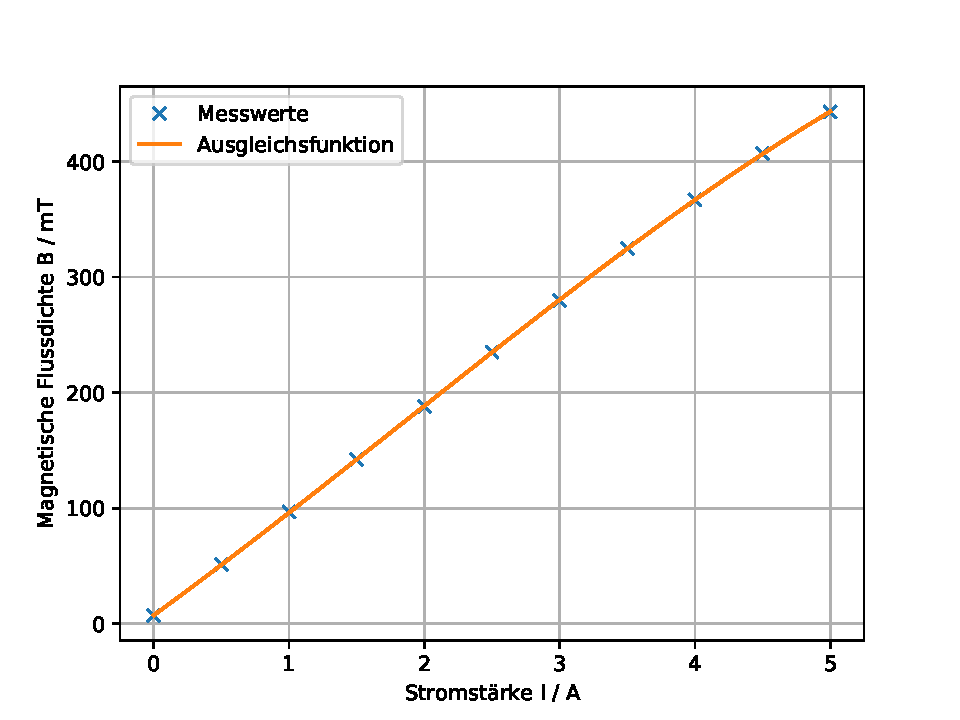
\includegraphics[width=\textwidth]{content/data/magnetfeld.pdf}
    \caption{Der angelegte Strom $I \, \text{in} \, \si\ampere}$ aufgetragen gegen die gemessene Magnetfeldstärke $B \, \text{in} \, \si{\milli\Tesla}$.}
    \label{fig:Magnetfeld}
\end{figure}

\subsection{Blaue Spektrallinie}
\subsubsection{$\pi -$Polarisiertes Licht}
Zunächst wurde wie im Abschnitt \ref{sec:Durchführung} beschrieben, die Änderung der blauen Spektrallinie im Magnetfeld aufgenommen.
Das Bild der Aufspaltung für das $\pi -$Polarisierte Licht ist dabei in Abbildung \ref{fig:pi-blau} zu sehen.
In der Grafik wurden die Blauen Spektrallinien ohne Einfluss durc ein Magnetfeld und die Spektrallinie des $\pi -$Polarisierten Lichts im Magnetfeld übereinander gelegt.
Oben befindet sich dabei das Licht welches durch das Magnetfeld beeinflusst wurde und unten das Licht welches nur durch durch das Prisma gebrochen wurde.

\begin{figure}
    \centering
    \includegraphics[width=\textwidth]{content/data/Blau_0_pi_uebereinander.JPG}
    \caption{Im oberen Teil des Bilder ist das $\pi -$Polarisierte Licht unter Einfluss des Zeeman-Effekts zu sehen. Im unteren Teil ist die blaue Spektrallinie der Lampe ohne Magnetfeld zum Vergleich zu sehen.}
    \label{fid:pi-blau}
\end{figure}

Zur Messung der Wellenlängenverschiebung wurden nun die Abstände zwischen Maxima und Maxima der unbeeinflussten Spektrallinien $\Delta \lambda$
und die Abstände zwischen den Anfängen der Maxima der durch den Zeeman-Effekt beeinflussten Maxima $\delta \lambda$ gemessen.
Die Längen wurden dabei in Anzahl von Pixeln gemessen und sind in der Tabelle \ref{tab:blau-pi} zu finden.

\begin{table}
    \centering
    \caption{Die Abstände der Maxima der Spektrallinien in Anzahl von Pixel.
    $\Delta \lambda$ gibt dabei die unbeeinflussten Abstände und $\delta \lambda$ die durch den Zeeman-Effekt beeinflussten Abstände, des $\pi -$ Polarisirtem Lichts an.}
    \begin{tabular}
        \toprule
        Ordnung & $\Delta \lambda$ & $\delta \lambda $  \\
        \midrule
        1  $    270 $   56  \\
        2  $    270 $   54  \\
        3  $    224 $   52  \\
        4  $    206 $   54  \\
        5  $    190 $   44  \\
        6  $    182 $   44  \\
        7  $    178 $   44  \\
        8  $    165 $   40  \\
        9  $    150 $   36  \\
        10 $    145 $   36  \\
        11 $    142 $   34  \\
    \end{tabular}
    \label{tab:blau-pi}
\end{table}

Um nun die Wellenlängenverschiebung zu berechnen wurde zunächst über alle Werte gemittlet und dann die Formel
\begin{equation}

    \label{eq:Wellenlängenverschiebung}
\end{equation}
genutzt.
Zudem wurde von einen systematische Fehler von $\pm 5$ Pixeln angenommen, da die Maxima der Spektrallinie im Programm Paint3D \cite{paint3d} abgeschätzt worden sind.
Zur Berechung der Fehler der Wellenlängenverschiebung wurde das Python Paket uncertainties \cite{uncertainties} genutzt.
Dieses nutzt zur Berechung der Fehlerfortpflanzung die Formel
\begin{equation}
    .
    \label{eq:fehler_Wellenlängenverschiebung}
\end{equation}
Die bestimmte Wellenlängenverschiebung beträgt

\begin{align*}
    \lambda _\text{$\pi$-blau} = & \SI{0.00316(011)}{\nano\meter} \\
\end{align*}

\subsubsection{$\sigma -$Polarisiertes Licht}

%Die selben Berechungen wurden für die Messwerte der $\sigma -$Spektrallinien des Blauen Lichts durchgeführt.
Die Aufspaltung der Maxima des Blauen Licht welches $\sigma -$Polarisiert ist, ist in Abbildung \ref{fig:sigma-blau} zu sehen.

\begin{figure}
    \centering
    \includegraphics[width=\textwidth]{content/data/Blau_0_sigma_uebereinander.JPG}
    \caption{Im oberen Teil des Bilder ist das $\sigma -$Polarisierte Licht unter Einfluss des Zeeman-Effekts zu sehen. Im unteren Teil ist die blaue Spektrallinie der Lampe ohne Magnetfeld zum Vergleich zu sehen.}
    \label{fig:sigma-blau}
\end{figure}

Zur Bestimmung der Wellenlängenverschiebung wurde wie beim $\pi -$Polarisiertem Licht zunächst $\Delta \lambda$ und $\delta \lambda$ gemessen.
Die gemessenen Werte sind in Tabelle \autoref{tab:blau-sigma} zu sehen.

\begin{table}
    \centering
    \caption{$\Delta \lambda$ der blauen Spektrallinie und $\delta \lambda$ des $\sigma -$Polarisiertem Lichts.}
    \begin{tabular}
        \toprule
        Ordnung & $\Delta \lambda$ & $\delta \lambda $  \\
        \midrule
        1   &   270  &    130   \\
        2   &   264  &    130   \\
        3   &   227  &    109   \\
        4   &   200  &    100   \\
        5   &   176  &    91    \\
        6   &   182  &    91    \\
        7   &   164  &    80    \\
        8   &   161  &    70    \\
        9   &   150  &    55    \\
        10  &   133  &    45    \\
        11  &   130  &    38    \\
        \bottomrule
    \end{tabular}
    \label{tab:blau-sigma}
\end{table}

Über Diese Werte $\Delta \lambda$ und $\delta \lambda$ in der Tabelle \autoref{tab:blau-sigma} wurde nun wieder gemittelt.
Dabei wurde wieder ein systematischer Fehler von $\pm 5$ Pixeln angenommen. 
Danach wurde nach Gleichung \eqref{eq:Wellenlängenverschiebung} die Wellenlängenverschiebung berechnet.
Hier wurde der Fehler wieder nach Gleichung \eqref{eq:fehler_Wellenlängenverschiebung} bestimmt.
Die Wellenlängenverschiebung des $\sigma -$Polarisiertem Lichts beträgt
\begin{align*}
    \lambda _\text{$\sigma$ -blau} =& \SI{0.00621(012)}{\nano\meter}
\end{align*}

\subsection{Rote Spektrallinie}
\subsubsection{$\sigma -$Polarisiertes Licht}
Zuletzt wurde die Aufspaltung von rotem Licht welches $\sigma -$Polarisiert ist aufgenommen.
Die Aufspaltung ist in der Abildung \autoref{fig:rot-sigma} zu erkennen.

\begin{figure}
    \centering
    \includegraphics[width=\textwidth]{content/data/Red_0_sigma_uebereinander.JPG}
    \caption{Im oberen Teil des Bilder ist das $\sigma -$Polarisierte Licht unter Einfluss des Zeeman-Effekts zu sehen. Im unteren Teil ist die rote Spektrallinie der Lampe ohne Magnetfeld zum Vergleich zu sehen.}
    \label{fig:rot-sigma}
\end{figure}

Es wurden die Werte $\Delta \lambda$ und $\delta \lambda$ bestimmt diese sind in Tabelle \autoref{tab:sigma-rot} zu sehen.

\begin{table}
    \centering
    \caption{$\Delta \lambda$ der roten Spektrallinie und $\delta \lambda$ des $\sigma -$Polarisiertem Lichts.}
    \begin{tabular}
        \toprule
        Ordnung & $\Delta \lambda$ & $\delta \lambda $  \\
        \midrule
        1   &   308  &    76    \\
        2   &   244  &    63    \\
        3   &   228  &    59    \\
        4   &   202  &    59    \\
        5   &   190  &    42    \\
        6   &   177  &    40    \\
        7   &   168  &    34    \\
        8   &   164  &    29    \\
        9   &   147  &    21    \\
        10  &   168  &    21    \\
        \bottomrule
    \end{tabular}
    \label{tab:sigma-rot}
\end{table}

Die Werte aus der Tabelle \autoref{tab:sigma-rot} wurden gemittelt worauf nach Gleichung \eqref{eq:Wellenlängenverschiebung} die Wellenlängenverschiebung berechnet wurde.
Es wurde ein systematische Fehler von $\pm 5$ Pixeln angenommen.
Die Wellenlängenverschiebung für die rote $\sigma -$Polarisierte Linie beträgt
\begin{align*}
    \lambda _\text{$\sigma$-rot} =&  \SI{0.00544(020)}{\nano\meter} \\
\end{align*}

Alle Wellenlängenverschiebung sind nocheinmal zusammengefasst in Tabelle \ref{tab:Wellenlängenverschiebung} zu sehen.

\begin{align}
    \lambda _\text{$\pi$-blau} = & \SI{0.00316(011)}{\nano\meter} \\
    \lambda _\text{$\sigma$ -blau} =& \SI{0.00621(012)}{\nano\meter}
    \lambda _\text{$\sigma$-rot} =&  \SI{0.00544(020)}{\nano\meter} \\
    \label{tab:Wellenlängenverschiebung_alle}
\end{align}

\subsection{Berechung der Landé-Faktoren}

Zur Berechung der Landé-Faktoren der verschieden Spektrallinie wird die Gleichung \eqref{eq:Lande_Faktor} genutzt.
